\chapter{Mesh related commands}


CNR  CERN 


%-----------------------------------------------------------------------
%-----------------------------------------------------------------------
%-----------------------------------------------------------------------

\section{Process of 3D meshes}

 {\tt MMVII} is not a point-cloud/mesh processing tool. However, during some devlopment, some
functionnalities appeared to be necessary and not easily accesible on open source.
As they may be usable in other context I describe them here.

%-----------------------------------------------------------------------
\subsection{MeshCheck}

\begin{verbatim}
 == Mandatory unnamed args : ==
  * string [FDP,Cloud] :: Name of input cloud/mesh
 == Optional named args : ==
  * [Name=Bin] bool :: Generate out in binary format ,[Default=false]
  * [Name=Out] string :: Name of output file if correction are done
  * [Name=Do2DC] bool :: check also as a 2D-triangulation (orientation) ,[Default=false]
  * [Name=Correct] bool :: Do correction, Defaut: Do It Out specified
\end{verbatim}

{\tt MicMac-V1} can generate mesh from a 3d point cloud with normal. For this it
uses the open source tool devlopped by M Kazhdan. Also this tool is robust,
it has sometime topologicall problem that can block further processing.
The command {\tt MeshCheck} has been developped to  detect and potentially
correct these problems.

The first problem detected   is the fact that the same point that is duplicate in
a single triangle  like $ABC$  with $P_A=P_B$. This point are detected and
if the option {\tt Correct} is activated, a graph-quotient algorithm is applied 
on point that are detected as multiple.

The second check is $3d$ surface orientatbility . A message indicating the detected
pair of adjacent triangle badly oriented is printed.  No correction is
done, because untill now no such problem was encounterred.

If the option {\tt Do2DC} is activated, the triangulation is considered
as a $2$ triangle (setting $z$ to $0$) and  the $2d$ orientation correctness is
tested (have all the triangle the same orientation).


%-----------------------------------------------------------------------
\subsection{MeshCloudClip}

\begin{verbatim}
 == Mandatory unnamed args : ==
  * string [FDP,Cloud] :: Name of input cloud/mesh
  * string [3DReg] :: Name of 3D masq

 == Optional named args : ==
  * [Name=Out] string :: Name of output file
  * [Name=Bin] bool :: Generate out in binary format ,[Default=false]
\end{verbatim}


The mesh generated by Poisson method generate a smooth extension of the surface
that can be problematic, for example in the surface devlopment process. This
commande allow to clip the mesh using a $3d$ region.  For now the region
must come in the {\tt MicMac-V1} format as seized by {\tt mm3d SaisieMasqQT}
as for now there is no well established format for $3d$ volumes.
Figure~\ref{fig:MeshClip} illustrate the result of {\tt MeshCloudClip}

\begin{figure}
\centering
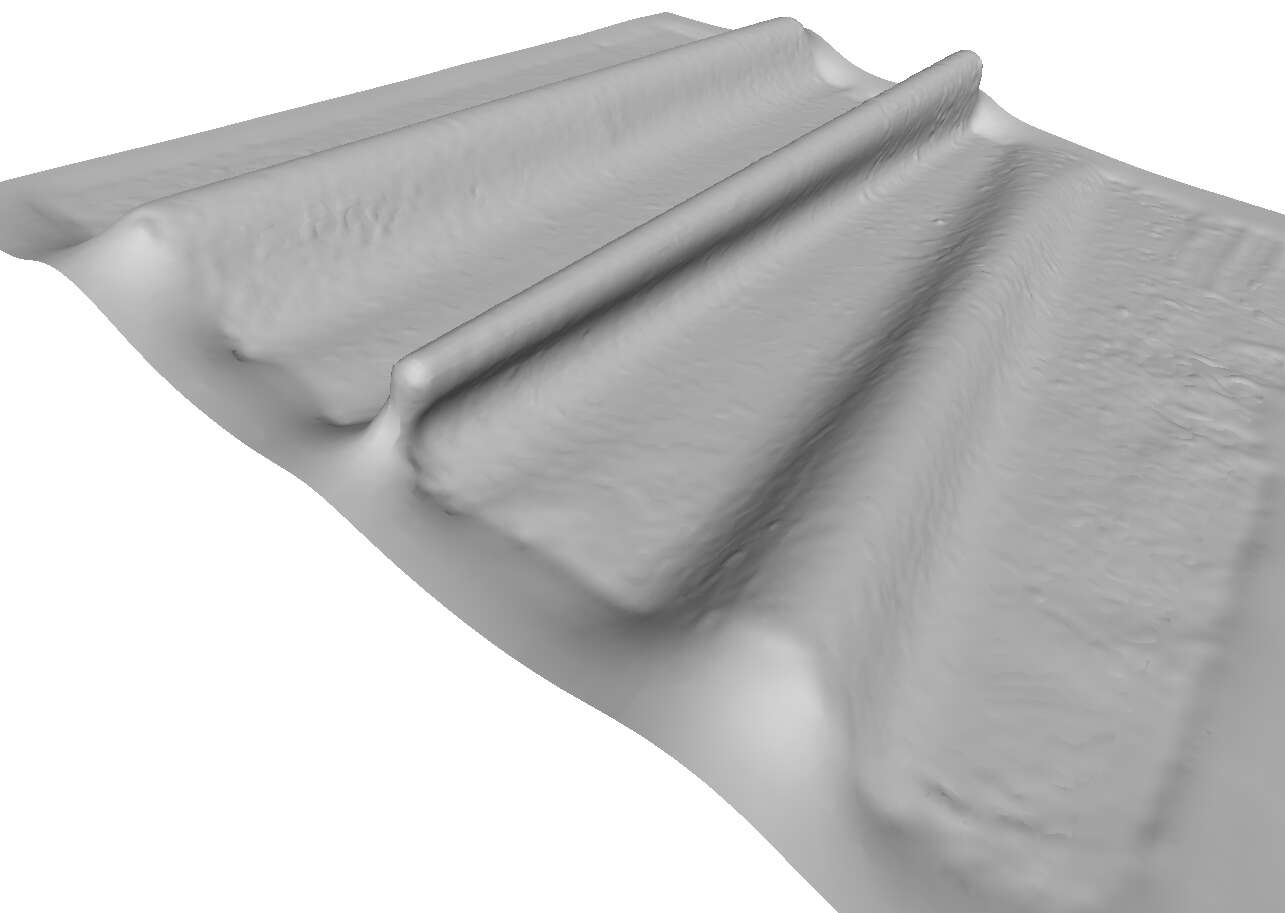
\includegraphics[width=6cm]{CommandReferences/ImagesComRef/MeshWithSkirt.jpg}
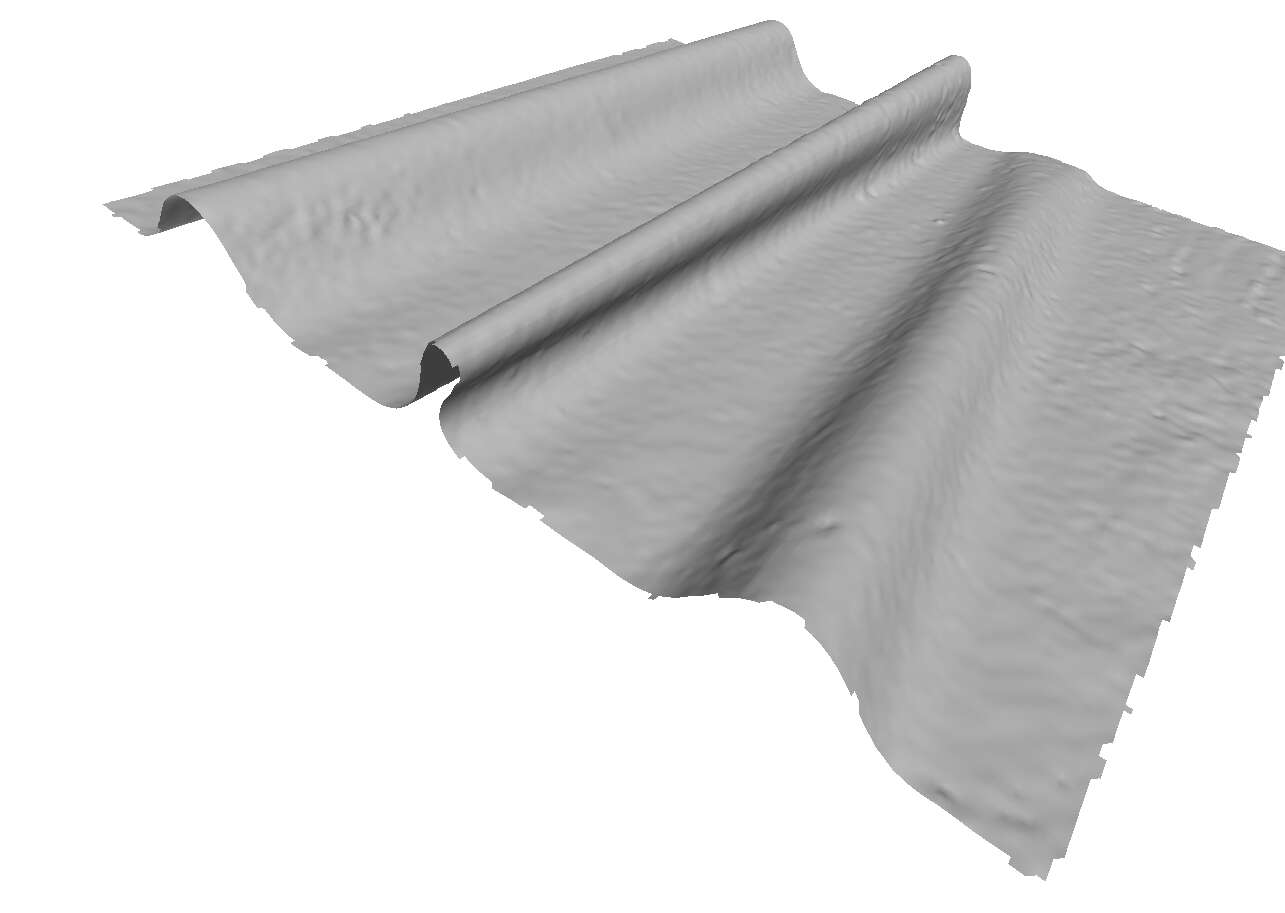
\includegraphics[width=6cm]{CommandReferences/ImagesComRef/MeshCliped.jpg}
\caption{Letft mesh with undesirable extension, right mesh after clipping}
\label{fig:MeshClip}
\end{figure}



%-----------------------------------------------------------------------
%-----------------------------------------------------------------------
%-----------------------------------------------------------------------

\section{Mesh development}

This section describe the tools that were devloped for surface devlopment.

%-----------------------------------------------------------------------
\subsection{MeshDevGen}
This "tiny" tool was made to check the correctness of the surface devlopment algorithm. 
It generate a synthetic mesh, that is completely devlopable and for with we
know the 2 devlopment. This surface is a $3$ extrusion of a logarithmic spiral.

Figure~\ref{fig:SpirAndDev} represent the 3D surface and its developped 2d surface.

\begin{figure}
\centering
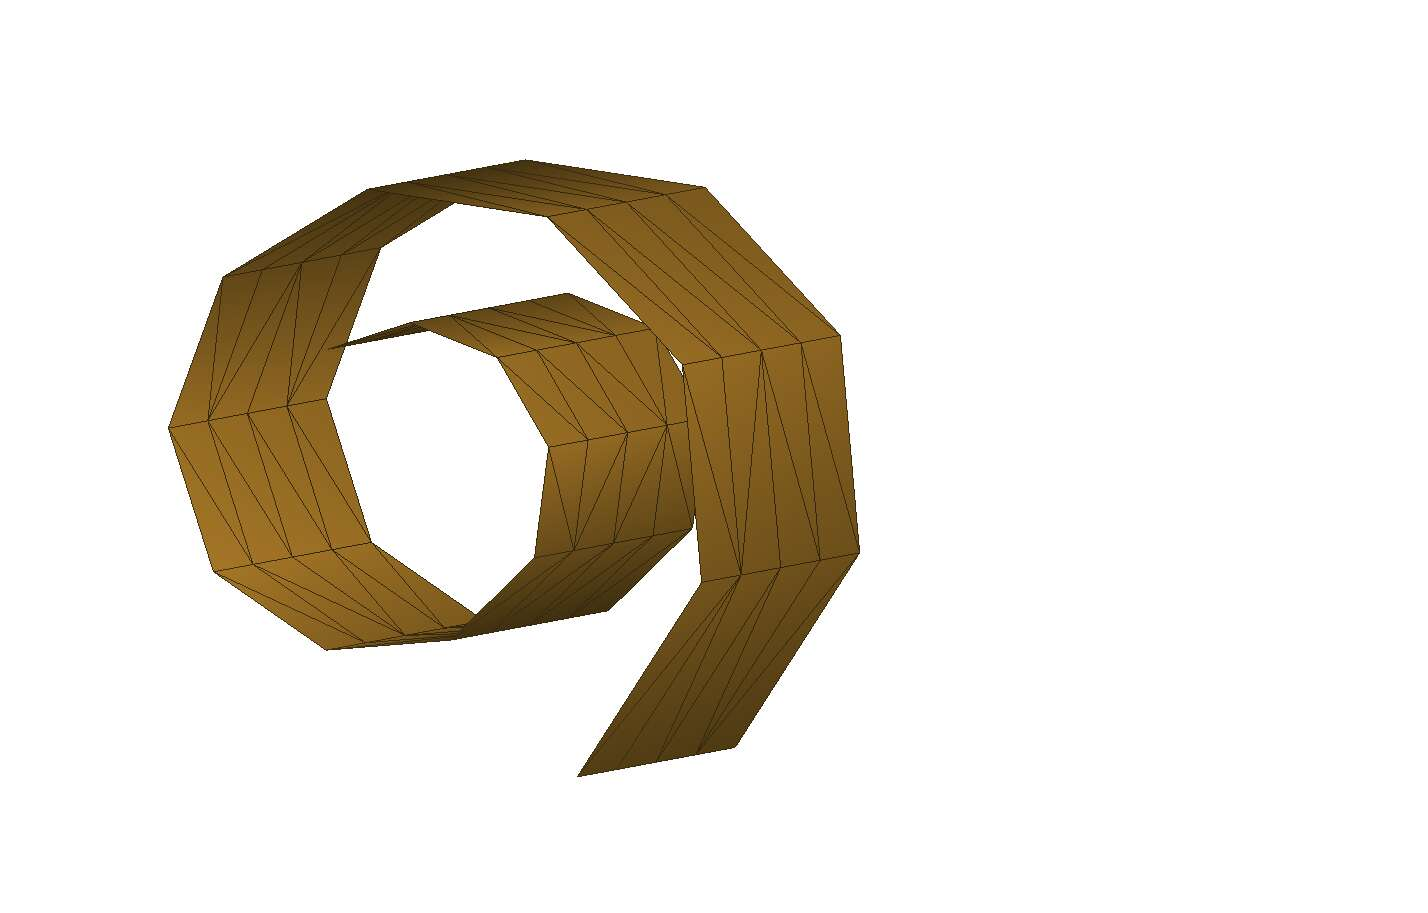
\includegraphics[width=6cm]{CommandReferences/ImagesComRef/Cyl3D01.jpg}
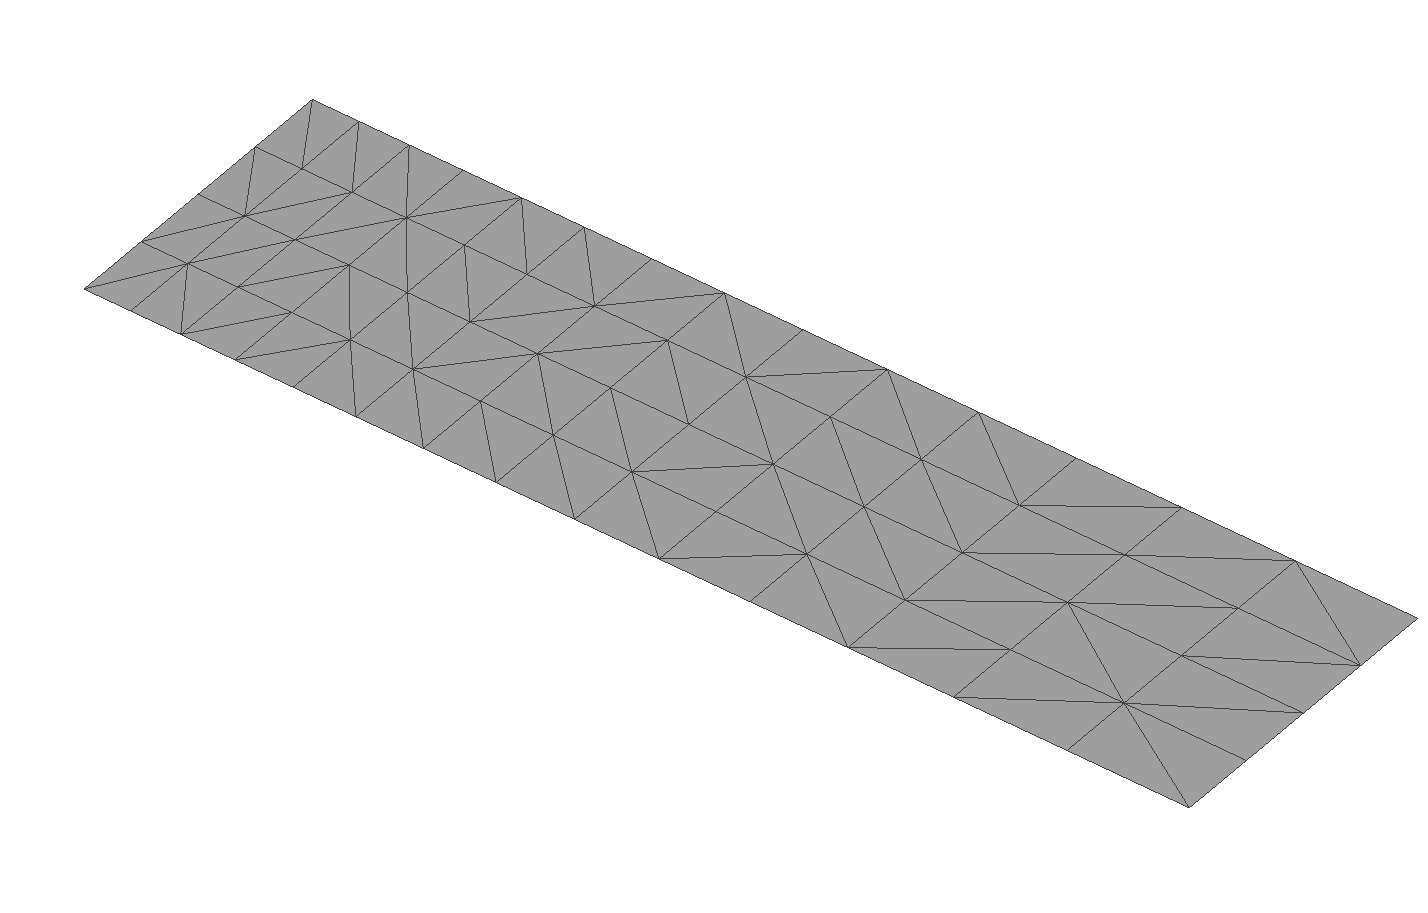
\includegraphics[width=6cm]{CommandReferences/ImagesComRef/CylDev00.jpg}
\caption{A synthetic 3D mesh, and its generated devloped surface}
\label{fig:SpirAndDev}
\end{figure}

%-----------------------------------------------------------------------
\subsection{MeshDev}

\begin{verbatim}
== Mandatory unnamed args : ==
  * string [FDP,Cloud] :: Name of input cloud/mesh
== Optional named args : ==
  * [Name=Out] string :: Name of output file
  * [Name=Bin] bool :: Generate out in binary format ,[Default=false]
  * [Name=NbCByS] int :: Number of compensation by step ,[Default=3]
  * [Name=ShowAv] bool :: Show advancement of computation ,[Default=true]
  * [Name=CheckReach] bool :: Check reached face&som at end ,[Default=true]
  * [Name=WDistE] double :: Weight on edge dist ,[Default=0]
  * [Name=WRot] double :: Weight on rot on 2d triangles ,[Default=1]
  * [Name=NbIE] int :: Number of iteration at end
\end{verbatim}

This tool is used to make the $2d$ development of a $3d$ surface. As the real surface
is generally not strictly devlopable, this is done by minimzing the energy of deformation.
The constraint is that the devlopment must be, as much as possible isometric (distance on
the plane is the same that geodetic distance on $3d$ surface).  More precisely :

\begin{itemize}
      \item let  $P_i$ be the $3d$ points of the triangulation, $P_i \in \RR^3$;
      \item let  $\phi(P_i)$ be unknown $2d$  position of the devlopment $\phi(P_i) \in \RR^2$;
      \item let  $\mathcal{T}_t = \{P_{t_1},P_{t_2},P_{t_3}\}, t \in [1,T] $ be the $T$ triangles;
\end{itemize}


The command offers different option corresponding to different formalization of the isometry.
The simpler is given by :

\begin{equation}
   E_d(\phi) =   \sum_{t=1}^T \sum_{m,n=1}^3  \{ d(P_{t_m},P_{t_m})-  d(\phi(P_{t_m}),\phi(P_{t_m})) \}  ^2
   \label{DevEqDist}
\end{equation}

For technicall reason (see paper to come) the equation~\ref{DevEqDist} is not stable and
the equation~\ref{Eq:MeshDev1T} is generally preferable.
For each triangle  $\mathcal{T}_t$ \emph{independantly} we can easily compute a \emph{perfect} development
in a $2d$ triangle $\mathcal{T}^2_k$= $q_{t_1},q_{t_2},q_{t_3}$, such that 
$d(q_{t_n},q_{t_m})=d(P_{t_m},P_{t_n}) \; m,n \in (1,2,3)$, so if the development
were perfect, there would exist for each triangle a rotation $R^t$ such that :

\begin{equation}
	\phi(P_{t_m}) =  R^t q^t_m  \;\; m \in (1,2,3) \label{Eq:MeshDev1T}
\end{equation}


Let note $\psi$ the application associate a rotation to each triangle $R^t = \psi(\mathcal{T}_t)=$.
We then try to compute simultaneously the $\phi$ and $\psi$ that minizes globaly the 
formula of equation~\ref{Eq:MeshDev1T} :

\begin{equation}
    E_R(\phi,\psi)= \sum_{t=1}^T \sum_{m=1}^3  d\{\phi(P_{t_m}) - \psi(\mathcal{T}_t)(q_{t_m})\} ^2
\end{equation}

%-----------------------------------------------------------------------

\subsection{MeshProjImage}

\begin{verbatim}
 == Mandatory unnamed args : ==
  * string [MPF0,FDP] :: Name of image
  * string [Cloud,In] :: Name of input cloud/mesh
  * string [Ori,In] :: Input Orientation
 == Optional named args : ==
  * [Name=M2] string [Cloud,In] :: Mesh 2D, dev of cloud 3D,to generate a visu of hiden part 
  * [Name=ResZBuf] double :: Resolution of ZBuffer ,[Default=3]
  * [Name=DoIm] bool :: Do images ,[Default=false]
  * [Name=NbPixIR] int :: Resolution of ZBuffer ,[Default=2000]
  * [Name=MII] double :: Margin Inside Image (for triangle validation) ,[Default=4]
  * [Name=SkWE] bool :: Skip command when result exist
  * [Name=OutRad] string [Rad,Out] :: Output Radiometry 
  * [Name=FFI0] string [FFI0] :: File Filter Interval, Main Set
\end{verbatim}


%-----------------------------------------------------------------------
\subsection{MeshImageDevlp}





